\section{Verifica}
	\subsection{Attività}
		\subsubsection{Analisi}
			Per poter determinare il livello di qualità del prodotto il team di sviluppo utilizza diversi tipi di tecniche di analisi dei dati.\\
			Queste possono essere suddivise in due grandi categorie:
			\begin{itemize}
				\item analisi statica;
				\item analisi dinamica.
			\end{itemize}
			\paragraph{Analisi statica}
				L'analisi statica è una forma di valutazione di un sistema o di un suo componente basato sulla sua forma, struttura, contenuto, documentazione senza che esso sia eseguito. Tali tecniche, dunque, sono applicabili tanto al codice quanto alla documentazione.
				Verranno usate le seguenti tecniche di analisi statica:
				\begin{description}
					\item[walkthrough] Tale tecnica viene utilizzata quando non si sa realmente cosa si sta cercando. Essa, infatti, consiste in una lettura da cima a fondo del documento/codice. Tale lettura ha lo scopo di trovare anomalie di qualsiasi tipo.
					\item[inspection] Tale tecnica viene utilizzata quando si ha un'idea di cosa si sta cercando e di cosa si potrebbe trovare. Essa consiste in una lettura mirata del documento/codice, sulla base di una lista degli errori comuni stilata in precedenza.
				\end{description}
				Applicare in modo fruttuoso la tecnica del walkthrough è molto oneroso e dispendioso. Tuttavia, quando non si possiede una lista degli	errori comuni (per esempio a inizio progetto), essa è l'unica soluzione. L'obiettivo è quello di formare una lista quanto più completa possibile di errori comuni in modo tale che possa essere eseguita quasi sempre la tecnica dell'inspection.
			\paragraph{Analisi dinamica}
				L'analisi dinamica è una forma di valutazione di un sistema software o di un suo componente basato sulla osservazione del suo comportamento in esecuzione. Tali tecniche, dunque, sono applicabili solo a componenti software e vengono svolte tramite l'esecuzione di test su essi.\\
				Deve essere preoccupazione di chi scrive i test fare in modo che essi siano di grande valore dimostrativo, in quanto il numero di test che devono essere effettuati è per forza di cose in numero finito e relativamente piccolo.
	\subsection{Procedure}
		\subsubsection{Verifica dei documenti}
			Dare inizio all'attività di verifica di un documento è compito del \insrole{Responsabile di Progetto}: esso assegna il compito a uno o più \insrole{Verificatori}. 
			Questi, con l'aiuto del diario delle modifiche, focalizzano la loro attenzione sulle sezioni del documento che sono state modificate.\\
			Per eseguire una verifica quanto più accurate e completa possibile è necessario controllare che sia stato rispettato quanto segue:
			\begin{enumerate}
				\item sintassi semplice e corretta;
				\item periodi brevi e leggibili;
				\item struttura del documento;
				\item norme tipografiche;
				\item proprietà di glossario.
			\end{enumerate}
			Durante l'esecuzione dell'intera procedura è importante che i \insrole{Verificatori} tengano traccia di tutti gli errori più comuni. In questo modo, 
			essi potranno essere riportati sulla lista di controlla necessaria per applicare in modo fruttuoso la tecnica dell'\textit{inspection}.
			
			\paragraph{Tracciamento degli errori pi\'u comuni nei documenti}
			Durante l'esecuzione dell'intera procedura di verifica dei documenti \'e importante che i \insrole{Verificatori} tengano traccia di tutti gli errori pi\'u comuni. \\
			\'E stata predisposta nell'applicativo Tracker una scheda con la possibilit\'a di vedere e gestire la lista di controllo. Durante la procedura il \insrole{Verificatore} andr\'a ad incrementare il counter della voce relativa all'errore trovato, contribuendo a creare una statistica degli errori. Ci sar\'a quindi la possibilit\'a per il \insrole{Responsabile di Progetto} di studiare l'andamento di questi ultimi e agire di conseguenza nel segnalare ai componenti del team eventuali situazioni particolarmente frequenti da evitare mentre si incrementano i documenti.\\
			Il tracciamento costruito appositamente permetter\'a sia di applicare in modo fruttuoso la tecnica dell'\textit{inspection} grazie alla lista di controllo, sia di migliorare la prevenzione sistematica degli errori pi\'u critici in fase di creazione dei documenti di progetto.
			\begin{figure}[H]
					\centering
					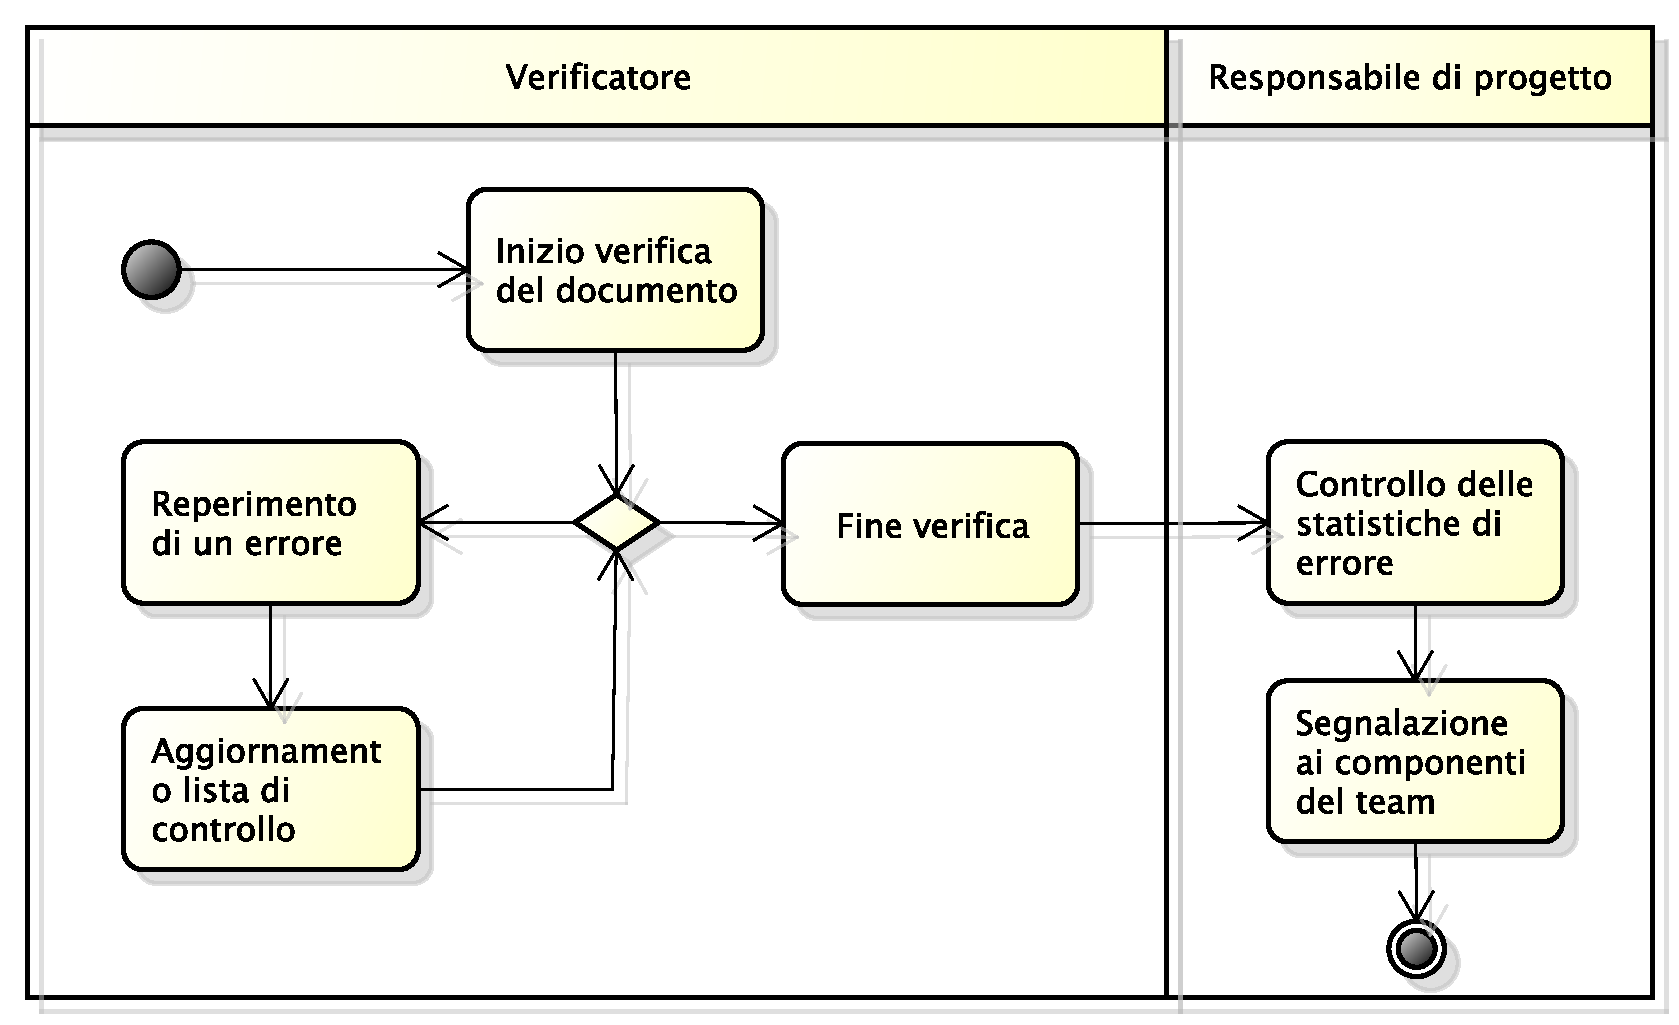
\includegraphics[width=0.6\textwidth]{NormeDiProgetto/Pics/ProceduraDecrementoErrori}
					\caption{Procedura per tracciamento errori comuni}
			\end{figure}
			
			\paragraph{Sintassi}
				I \insrole{Verificatori} devono preoccuparsi di individuare gli errori sintattici all'interno dei testi del documento. Tale compito può essere in 
				parte attuato tramite strumenti automatici (vedi sezione 6.3 del presente documento). È tuttavia necessario che un documento sia sempre sottoposto a \textit{walkthrough}, in quanto gli strumenti automatici non sono in grado di individuare parole corrette che sono utilizzate al di fuori del loro contesto.\\
				Inoltre, i \insrole{Verificatori} devono cercare tutte quelle parole che sono poco frequenti o comunque complesse (possono generare fraintendimenti o incomprensioni): va applicata la tecnica del \textit{walkthrough}.
			\paragraph{Periodi lunghi}
				I \insrole{Verificatori} devono calcolare l'indice Gulpease del documento (utilizzando l'appostio strumento automatico, vedi sezione 6.3 del presente documento). Qualora si ottenga un risultato inferiore alle aspettative si deve applicare il \textit{walkthrough} all'interno del documento: l'obiettivo deve essere quello di individuare frasi troppo lunghe (e che dunque possono essere di difficile comprensione e/o scarsa leggibilità).
			\paragraph{Struttura del documento}
				I \insrole{Verificatori} controllano con l'ausilio di strumenti automatici (vedi sezione 6.3 del presente documento) che la struttura del documento rispetti quanto descritto nel presente documento.
			\paragraph{Norme tipografiche}
				Nel presente documento sono state definite delle norme tipografiche di carattere generale. Molte di esse sono verificabili tramite strumenti automatici (vedi sezione 6.3 del presente documento). Per le restanti è necessario che i \insrole{Verificatori} applichino una fra le tecniche di inspection e \textit{walkthrough}	(si preferisce la prima nel momento in cui tramite la lista di controllo si riesce a trovare la grande maggioranza degli errori).
			\paragraph{Proprietà di glossario}
				È necessario che tutte le parole presenti all'interno del \insdoc{Glossario} siano marcate appropriatamente (come descritto nel presente 
				documento). Ciò viene fatto con l'ausilio di strumenti automatici (vedi sezione 6.3 del presente documento). Inoltre, è compito dei \insrole{Verificatori} trovare tutti quei termini che dovrebbero essere inclusi nel \insdoc{Glossario} ma che ancora non lo sono. Per tale compito si deve utilizzare \textit{walthrough} delle sezioni che sono state soggette a modifica prima dell'ultima verifica.
		\subsubsection{Verifica dei diagrammi UML}
			I Verificatori hanno il compito di controllare tutti i diagrammi UML che sono stati prodotti. I diagrammi utilizzati fino a questo momento 
			sono i seguenti:
			\begin{itemize}
				\item diagrammi dei casi d'uso;
				\item diagrammi di attività.
			\end{itemize}
			\paragraph{Diagrammi dei casi d'uso}
				Le verifiche che devono essere effettuate riguardano sostanzialmente i casi d'uso e gli attori.\\
				Innanzitutto si deve controllare se un attore è davvero tale. Per fare questo può essere utile porsi domande descritte in seguito.
				\begin{enumerate}
					\item Il presunto attore in questione è una persona che interagisce con il sistema? Se la risposta è si allora esso probabilmente è un attore, se la risposta è no passare al punto due.
					\item Sono in grado di modificare il presunto attore all'interno del mio sistema? Se la risposta è no allora probabilmente è un attore, se la risposta è si allora probabilmente non si tratta di un attore.
				\end{enumerate}
				\begin{figure}[H]
					\centering
					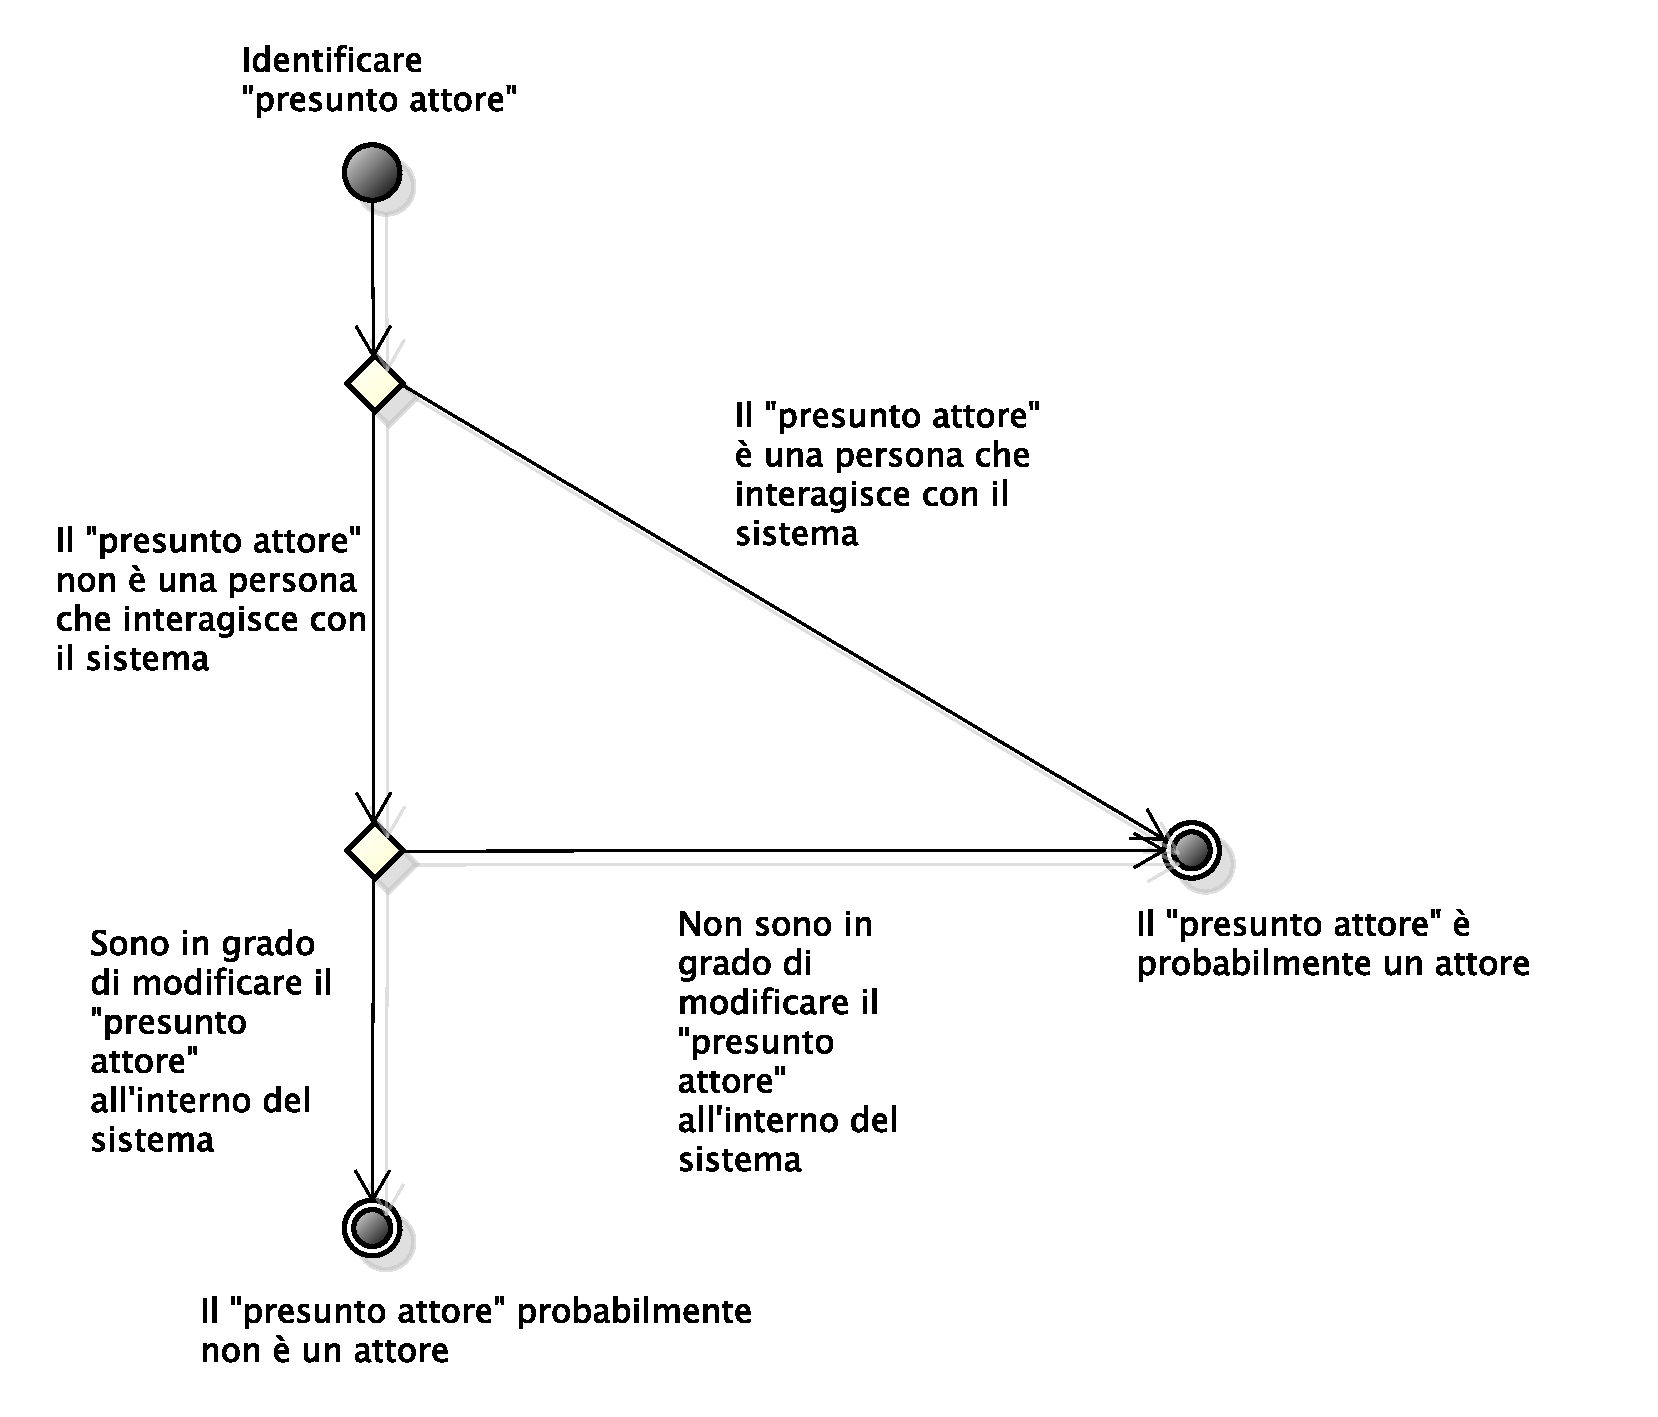
\includegraphics[width=0.6\textwidth]{NormeDiProgetto/Pics/VerificaAttori}
					\caption{Procedura per identificare un attore}
				\end{figure}
				Per quanto riguarda i casi d'uso, si controlla innanzitutto che siano utilizzate secondo lo standard UML le seguenti relazioni:
				\begin{itemize}
					\item inclusioni;
					\item generalizzazioni;
					\item estensioni
				\end{itemize}
				Infine, assicurarsi che i casi d'uso descrivano cosa il sistema fa e non cosa non fa.
			\paragraph{Diagrammi di attività}
				I diagrammi delle attività allo stato attuale delle cose sono stati usati esclusivamente per creare figure facilmente comprensibili che illustrino le procedure contenute nel presente documento. È dunque necessario verificare unicamente che tali diagrammi siano conformi allo standard UML.
	\subsection{Strumenti}
		In questa sezione vengono descritti gli aspetti essenziali degli strumenti che i Verificatori hanno a disposizione.
		\begin{description}
			\item[OrtographicCheck] Questo script sfrutta il software GNU Aspell per eseguire il controllo ortografico di un documento.
			\item[Gulpease] Questo script estrae il testo da un documento e ne calcola l'indice di leggibilità Gulpease.
			\item[NonBreakingSpaceCheck] Questo script controlla che un numero formattato secondo lo standard [SI/ISO 31-0] utilizzi lo spazio unificatore e non quello normale (errore in cui è facile incorrere).
		\end{description}